\begin{figure}
\center

	\begin{subfigure}[b]{0.4\textwidth}
		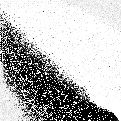
\includegraphics[height=0.23\textheight]{images/findings/round1/strategies_handmaxmin_pone.png}
		\caption{\handmaxmin}
	\end{subfigure}
	~
	\begin{subfigure}[b]{0.4\textwidth}
		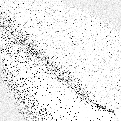
\includegraphics[height=0.23\textheight]{images/findings/round1/strategies_handmaxavg_pone.png}
		\caption{\handmaxavg}
	\end{subfigure}

	\begin{subfigure}[b]{0.4\textwidth}
		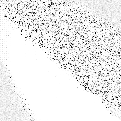
\includegraphics[height=0.23\textheight]{images/findings/round1/strategies_handmaxmed_pone.png}
		\caption{\handmaxmed}
	\end{subfigure}
	~
	\begin{subfigure}[b]{0.4\textwidth}
		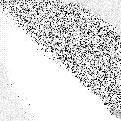
\includegraphics[height=0.23\textheight]{images/findings/round1/strategies_handmaxposs_pone.png}
		\caption{\handmaxposs}
	\end{subfigure}

	\begin{subfigure}[b]{0.4\textwidth}
		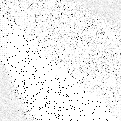
\includegraphics[height=0.23\textheight]{images/findings/round1/strategies_cribminavg_pone.png}
		\caption{\cribminavg}
	\end{subfigure}
	~
	\begin{subfigure}[b]{0.4\textwidth}
		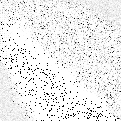
\includegraphics[height=0.23\textheight]{images/findings/round1/strategies_peggingmaxavggained_pone.png}
		\caption{\peggingmaxavggained}
	\end{subfigure}

	\begin{subfigure}[b]{0.4\textwidth}
		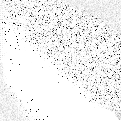
\includegraphics[height=0.23\textheight]{images/findings/round1/strategies_peggingmaxmedgained_pone.png}
		\caption{\peggingmaxmedgained}
	\end{subfigure}
	~
	\begin{subfigure}[b]{0.4\textwidth}
		
\includegraphics[height=0.23\textheight]{images/findings/round1/strategies_peggingminavggiven_pone.png}
		\caption{\peggingminavggiven}
	\end{subfigure}

\caption{
	All final strategy strengths for Agent 0
	when playing as the pone
	after training for one million games during Round 1.
}
\label{fig_r1-strats}
\end{figure}

